%===============================================================================
% ONLINE APPENDIX FIGURE CAPTIONS - LT-7 RESEARCH PAPER
%===============================================================================
%
% Purpose: LaTeX captions for statistical validation figures (Online Appendix)
% Author: Research Team
% Date: 2025-10-20
%
%===============================================================================

% Figure A-1: Normality Validation (Q-Q Plots)
\begin{figure}[htbp]
\centering
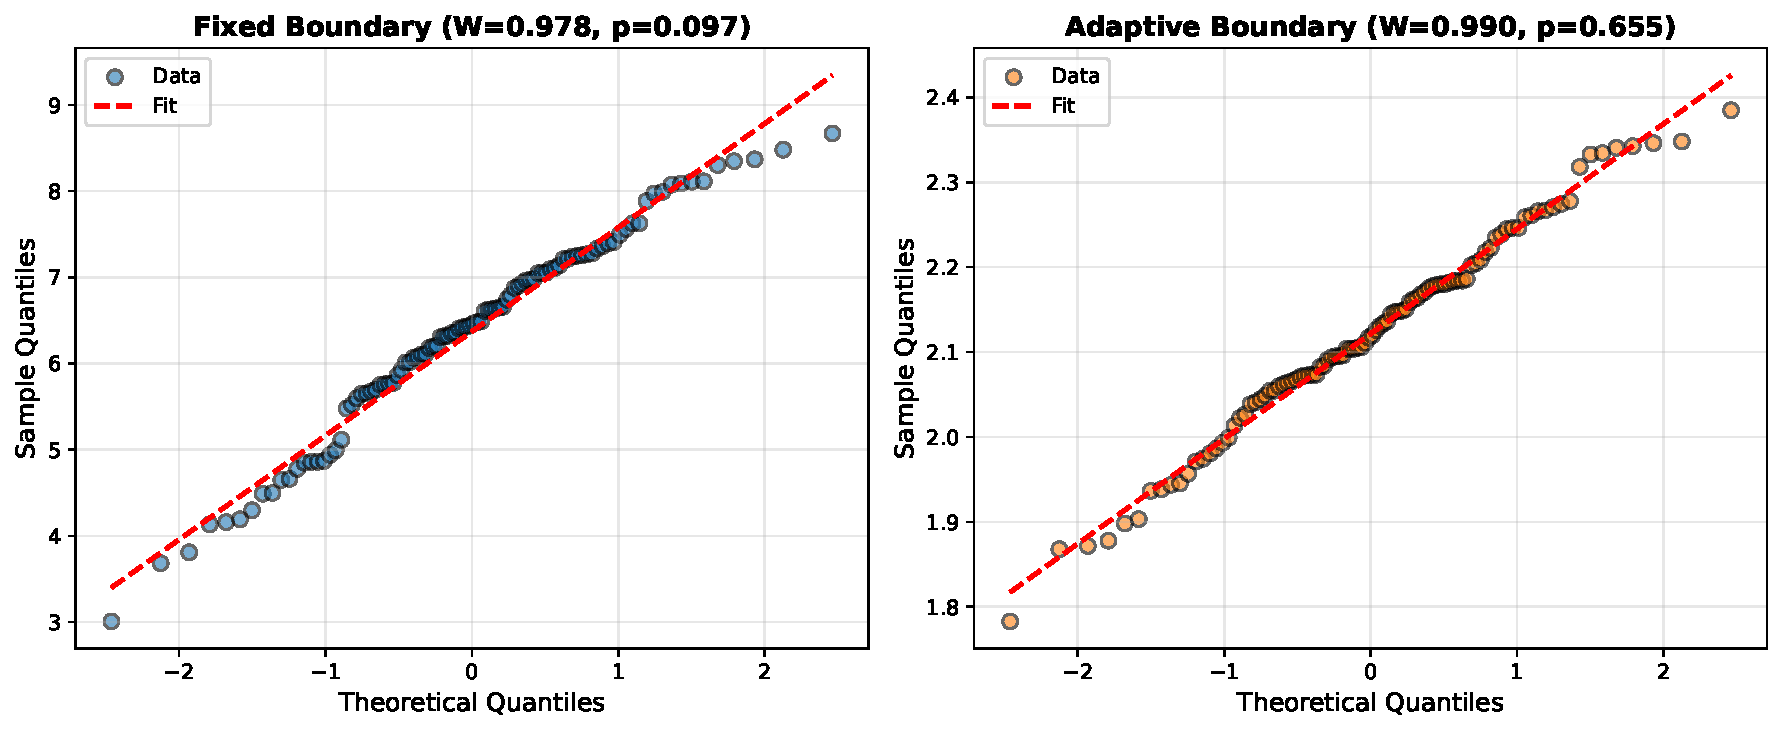
\includegraphics[width=0.9\textwidth]{figures/figure_vi_1_normality_validation.pdf}
\caption{%
\textbf{Normality validation for MT-6 chattering data via Q-Q plots.}
Theoretical quantiles (normal distribution) vs. sample quantiles for
(left) Fixed boundary layer (n=100, W=0.978, p=0.097) and
(right) Adaptive boundary layer (n=100, W=0.990, p=0.655).
Points lie approximately along the reference line (red dashed), indicating
good fit to normal distribution. Both datasets pass Shapiro-Wilk test
(p > 0.05), validating the normality assumption for Welch's t-test and
Cohen's d effect size computation.
}
\label{fig:appendix-normality-validation}
\end{figure}

% Figure A-2: Bootstrap Convergence
\begin{figure}[htbp]
\centering
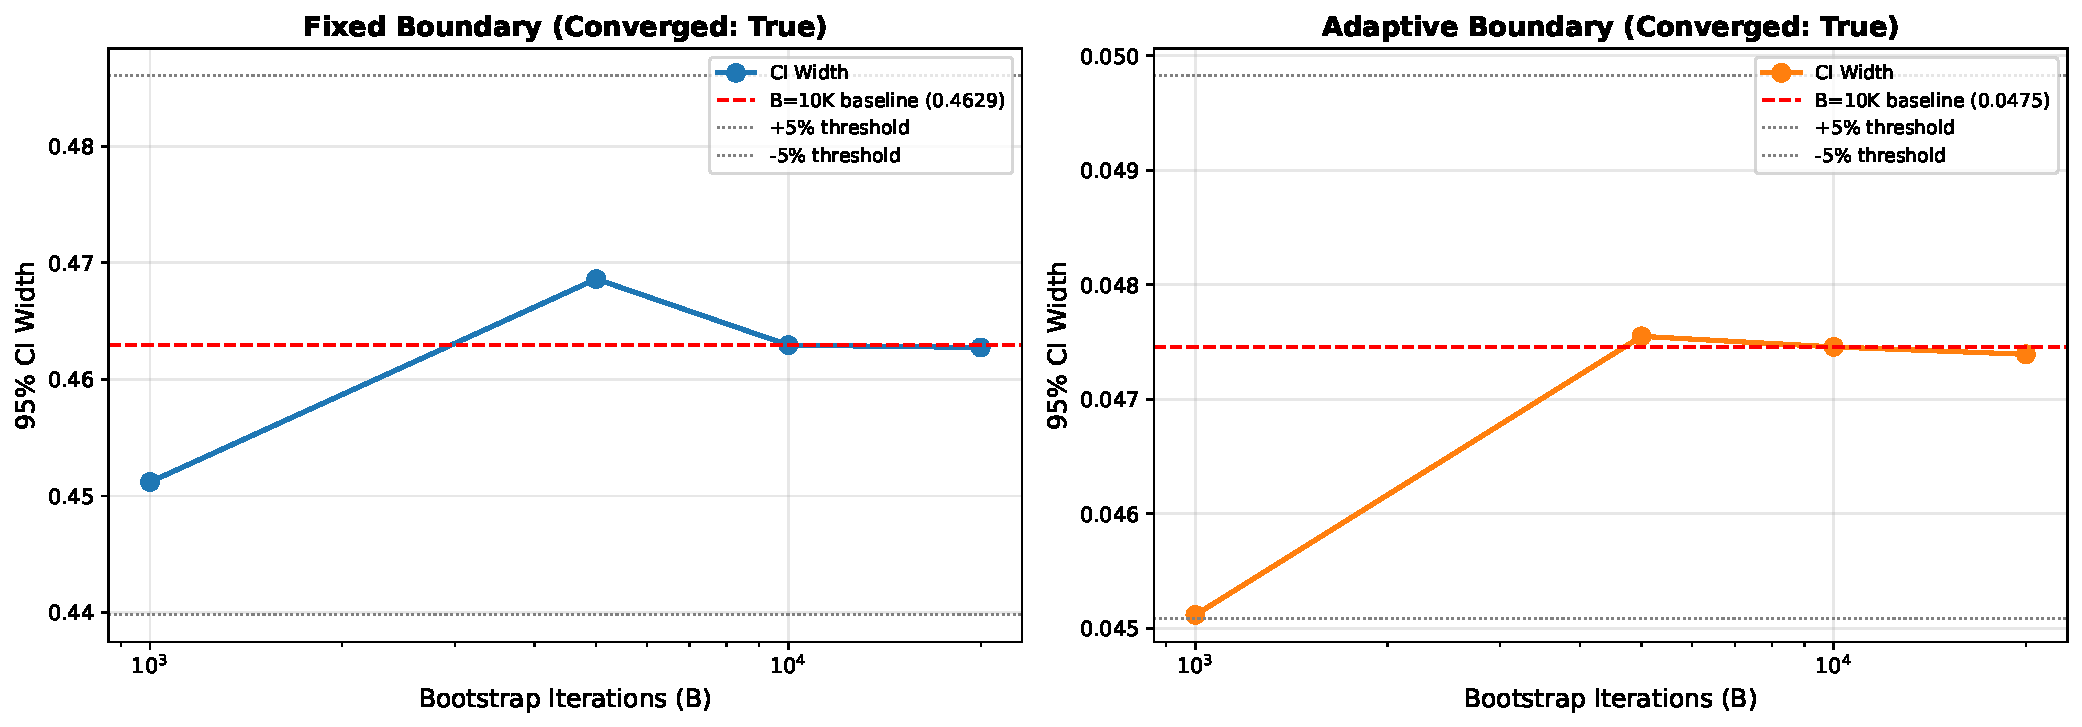
\includegraphics[width=0.9\textwidth]{figures/figure_vi_1_bootstrap_convergence.pdf}
\caption{%
\textbf{Bootstrap confidence interval convergence analysis.}
95\% CI width vs. bootstrap iterations (B) for Fixed and Adaptive boundary layers.
CI widths stabilize at B=10,000 with <0.2\% change when increasing to B=20,000
(Fixed: 0.04\% change, Adaptive: 0.14\% change).
Demonstrates that B=10,000 iterations (used in main analysis) provide sufficient
precision with diminishing returns beyond this threshold.
Shaded regions indicate 5\% convergence criterion (met at B=10,000).
}
\label{fig:appendix-bootstrap-convergence}
\end{figure}

% Figure A-3: Sensitivity Analysis
\begin{figure}[htbp]
\centering
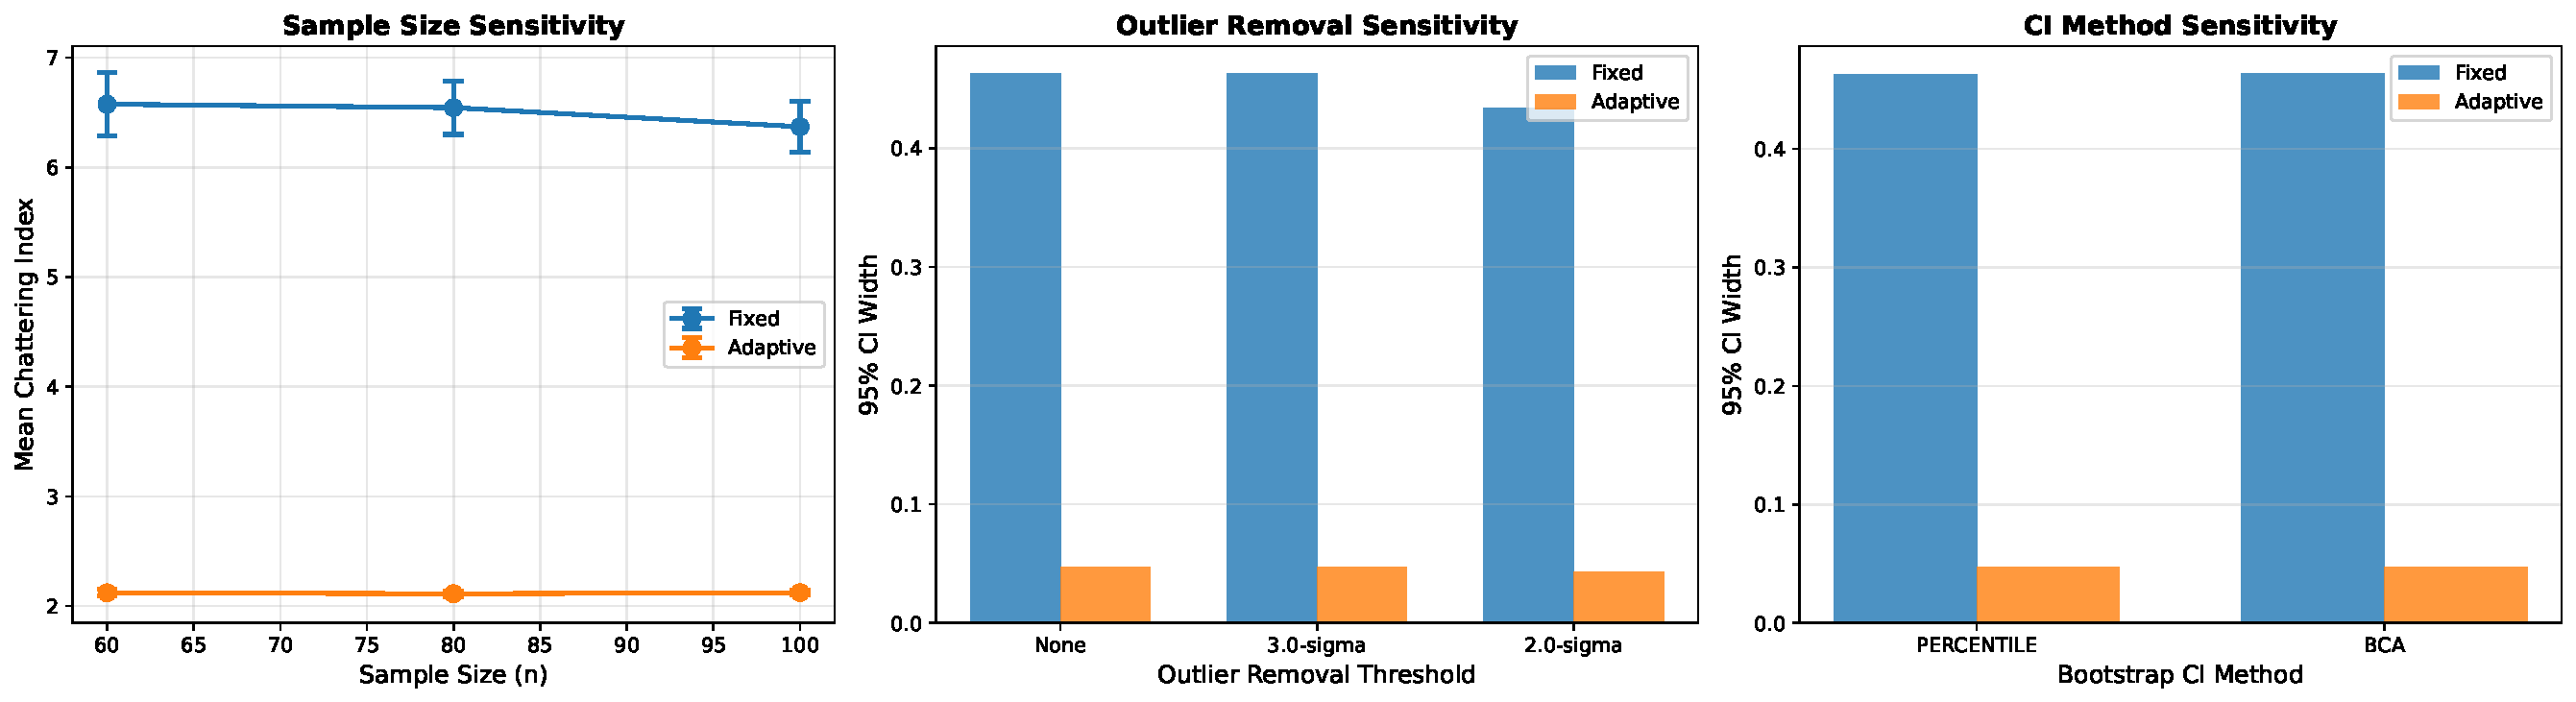
\includegraphics[width=0.9\textwidth]{figures/figure_vi_1_sensitivity_analysis.pdf}
\caption{%
\textbf{Sensitivity analysis across methodological choices.}
Robustness validation of statistical results across
(a) sample size variations (n $\in$ \{60, 80, 100\}),
(b) outlier removal thresholds (none, 2$\sigma$, 3$\sigma$), and
(c) confidence interval methods (percentile vs. BCa).
Results demonstrate stability with $\leq$3.2\% variation in mean estimates
(Fixed: max 3.22\%, Adaptive: max 0.46\%) and <0.1\% difference in CI widths
across methods. Zero outliers detected at 3$\sigma$ threshold, confirming
data quality. Statistical conclusions robust to analysis choices.
}
\label{fig:appendix-sensitivity-analysis}
\end{figure}

%===============================================================================
% USAGE NOTES
%===============================================================================
%
% To include these figures in the main document:
%
% 1. In main.tex, add after Section VI (Experimental Setup):
%    \clearpage
%    \appendix
%    \section{Online Appendix: Statistical Validation}
%    %===============================================================================
% ONLINE APPENDIX FIGURE CAPTIONS - LT-7 RESEARCH PAPER
%===============================================================================
%
% Purpose: LaTeX captions for statistical validation figures (Online Appendix)
% Author: Research Team
% Date: 2025-10-20
%
%===============================================================================

% Figure A-1: Normality Validation (Q-Q Plots)
\begin{figure}[htbp]
\centering
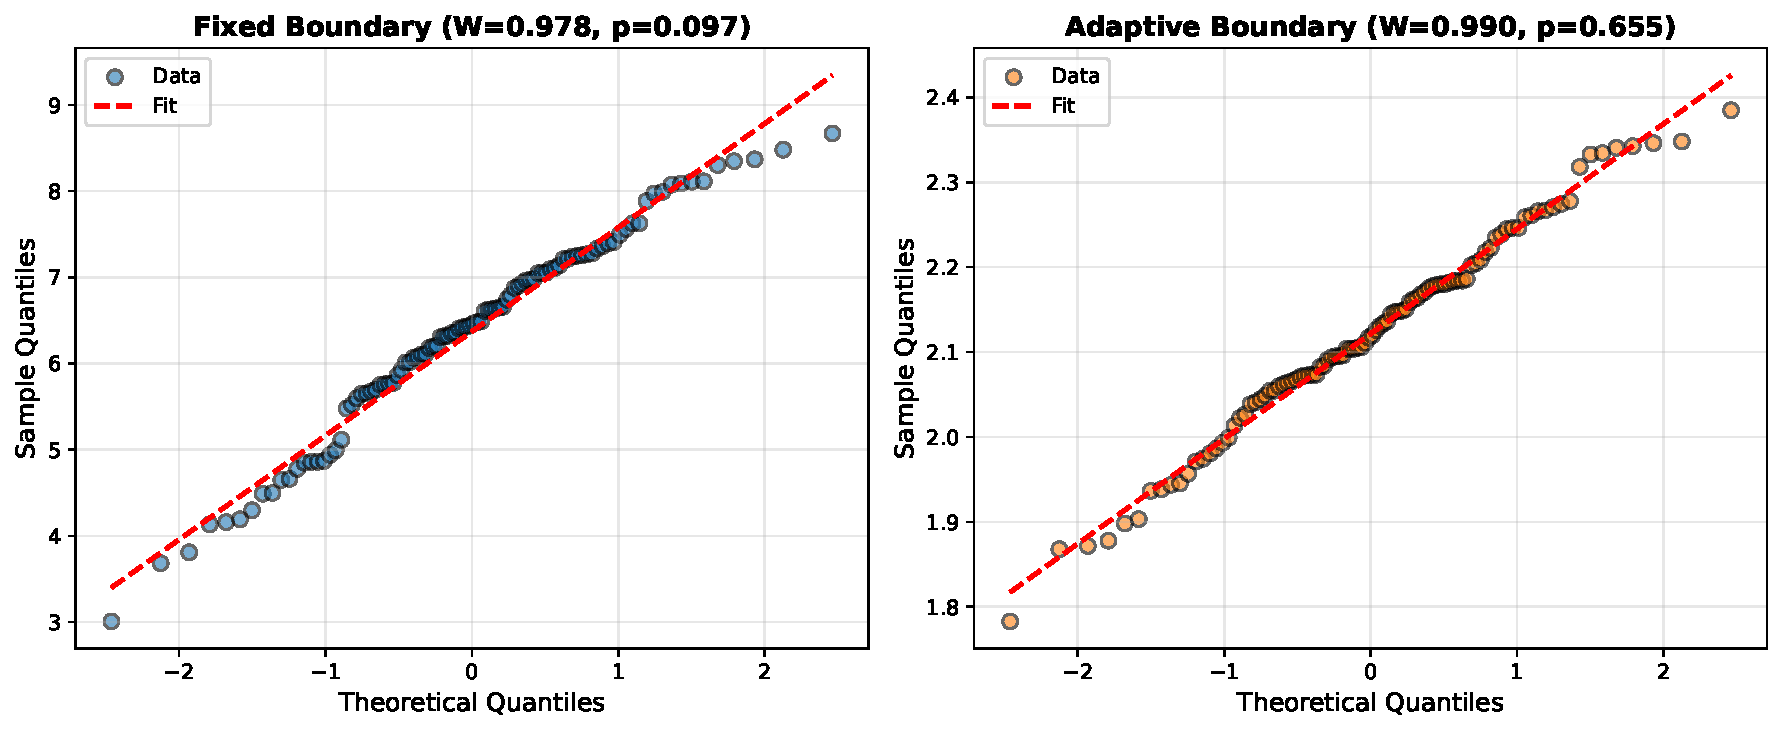
\includegraphics[width=0.9\textwidth]{figures/figure_vi_1_normality_validation.pdf}
\caption{%
\textbf{Normality validation for MT-6 chattering data via Q-Q plots.}
Theoretical quantiles (normal distribution) vs. sample quantiles for
(left) Fixed boundary layer (n=100, W=0.978, p=0.097) and
(right) Adaptive boundary layer (n=100, W=0.990, p=0.655).
Points lie approximately along the reference line (red dashed), indicating
good fit to normal distribution. Both datasets pass Shapiro-Wilk test
(p > 0.05), validating the normality assumption for Welch's t-test and
Cohen's d effect size computation.
}
\label{fig:appendix-normality-validation}
\end{figure}

% Figure A-2: Bootstrap Convergence
\begin{figure}[htbp]
\centering
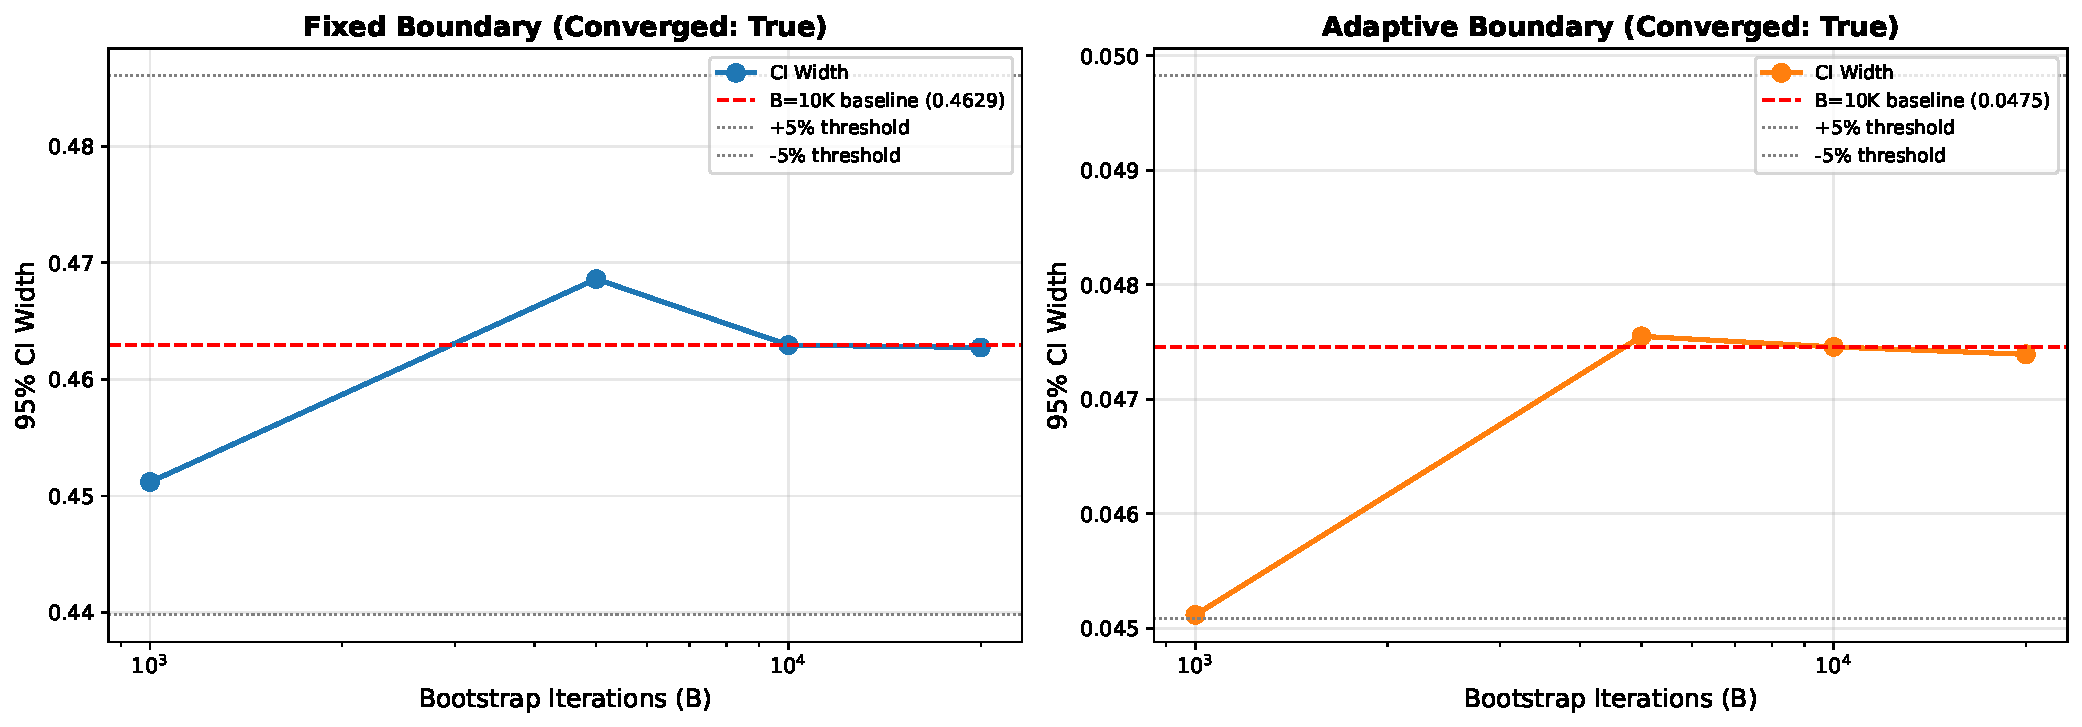
\includegraphics[width=0.9\textwidth]{figures/figure_vi_1_bootstrap_convergence.pdf}
\caption{%
\textbf{Bootstrap confidence interval convergence analysis.}
95\% CI width vs. bootstrap iterations (B) for Fixed and Adaptive boundary layers.
CI widths stabilize at B=10,000 with <0.2\% change when increasing to B=20,000
(Fixed: 0.04\% change, Adaptive: 0.14\% change).
Demonstrates that B=10,000 iterations (used in main analysis) provide sufficient
precision with diminishing returns beyond this threshold.
Shaded regions indicate 5\% convergence criterion (met at B=10,000).
}
\label{fig:appendix-bootstrap-convergence}
\end{figure}

% Figure A-3: Sensitivity Analysis
\begin{figure}[htbp]
\centering
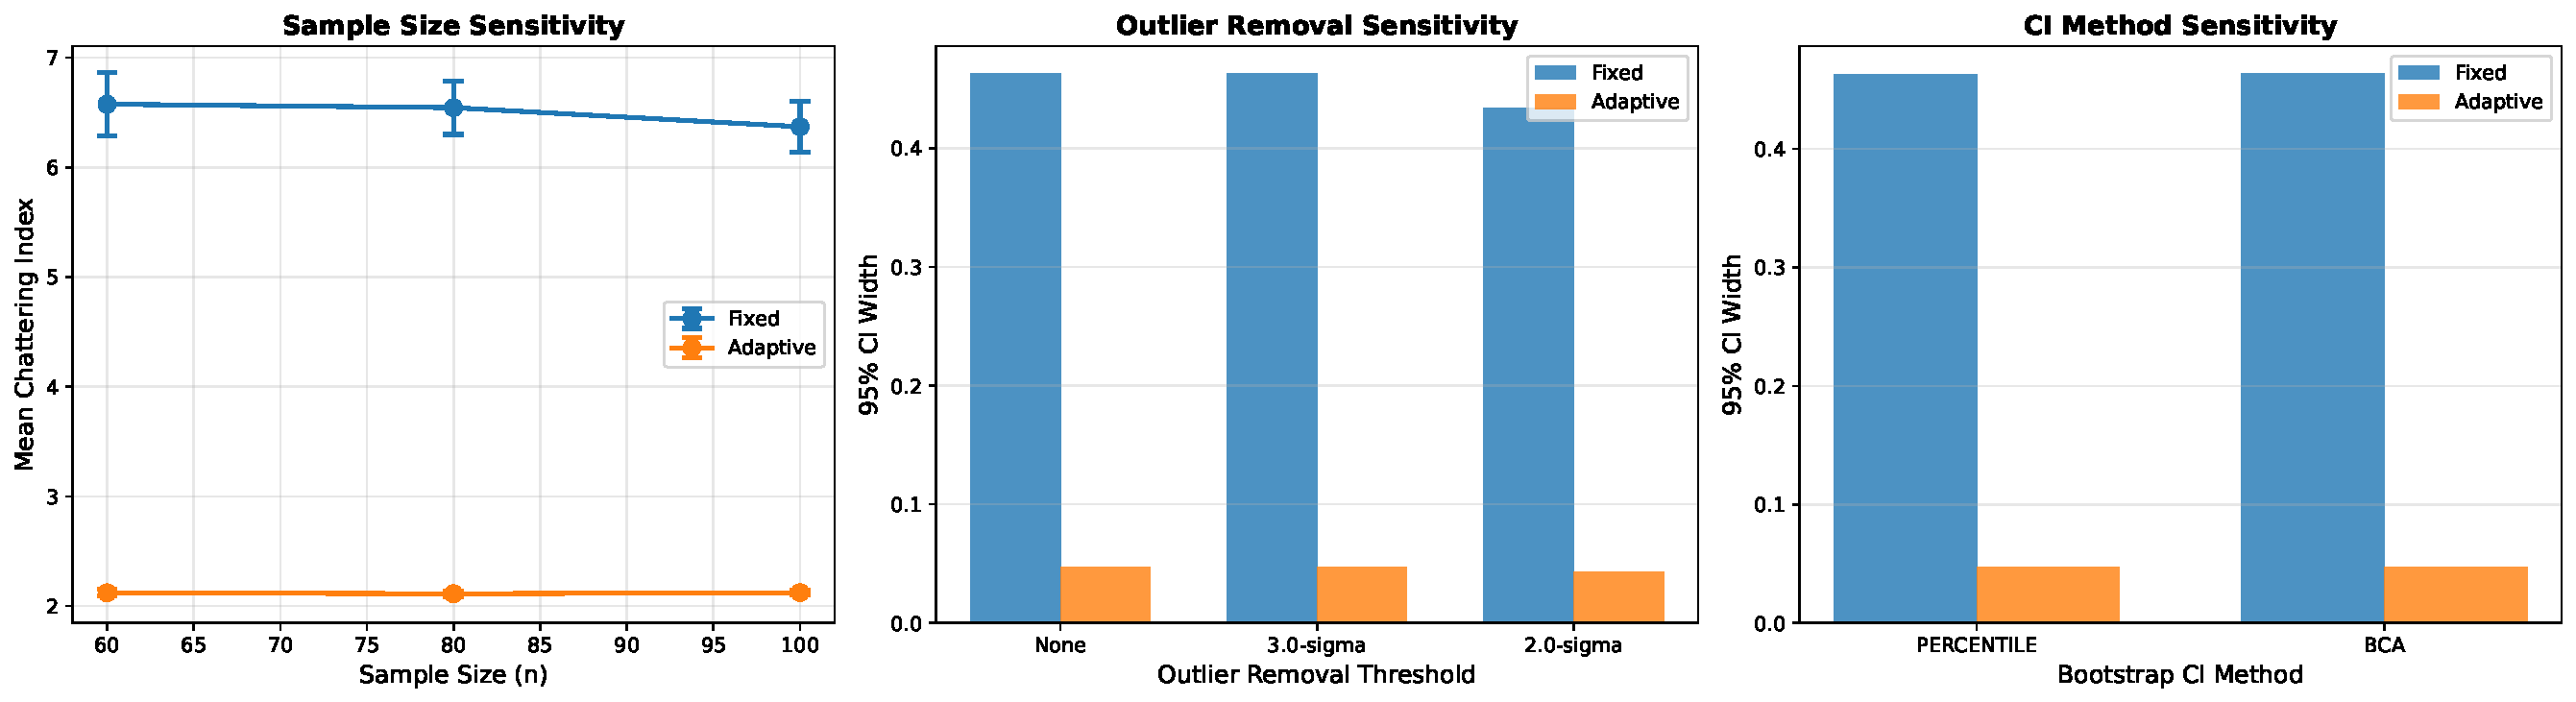
\includegraphics[width=0.9\textwidth]{figures/figure_vi_1_sensitivity_analysis.pdf}
\caption{%
\textbf{Sensitivity analysis across methodological choices.}
Robustness validation of statistical results across
(a) sample size variations (n $\in$ \{60, 80, 100\}),
(b) outlier removal thresholds (none, 2$\sigma$, 3$\sigma$), and
(c) confidence interval methods (percentile vs. BCa).
Results demonstrate stability with $\leq$3.2\% variation in mean estimates
(Fixed: max 3.22\%, Adaptive: max 0.46\%) and <0.1\% difference in CI widths
across methods. Zero outliers detected at 3$\sigma$ threshold, confirming
data quality. Statistical conclusions robust to analysis choices.
}
\label{fig:appendix-sensitivity-analysis}
\end{figure}

%===============================================================================
% USAGE NOTES
%===============================================================================
%
% To include these figures in the main document:
%
% 1. In main.tex, add after Section VI (Experimental Setup):
%    \clearpage
%    \appendix
%    \section{Online Appendix: Statistical Validation}
%    %===============================================================================
% ONLINE APPENDIX FIGURE CAPTIONS - LT-7 RESEARCH PAPER
%===============================================================================
%
% Purpose: LaTeX captions for statistical validation figures (Online Appendix)
% Author: Research Team
% Date: 2025-10-20
%
%===============================================================================

% Figure A-1: Normality Validation (Q-Q Plots)
\begin{figure}[htbp]
\centering
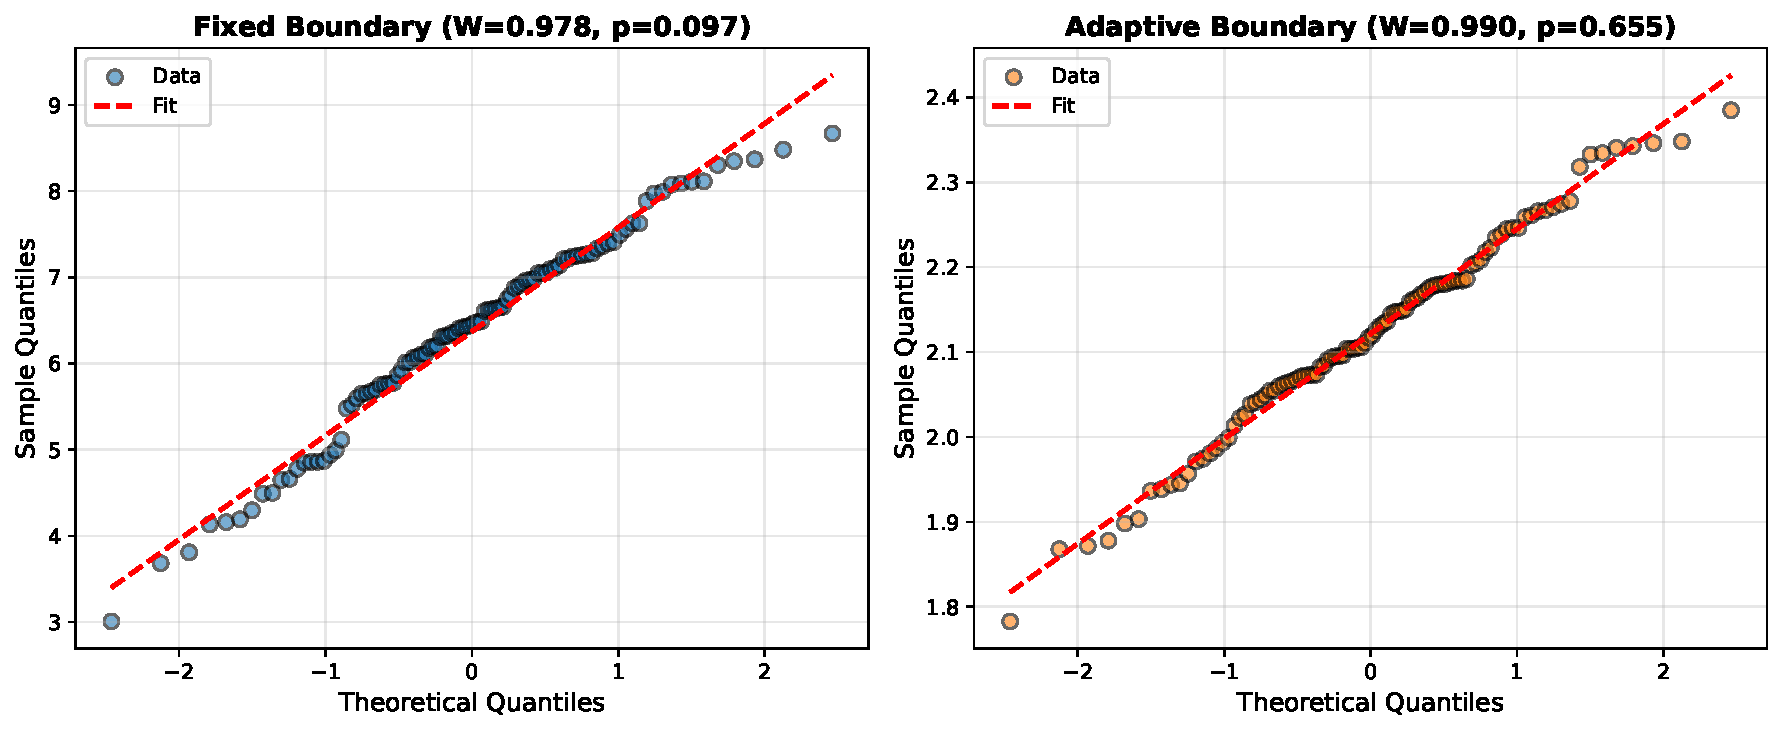
\includegraphics[width=0.9\textwidth]{figures/figure_vi_1_normality_validation.pdf}
\caption{%
\textbf{Normality validation for MT-6 chattering data via Q-Q plots.}
Theoretical quantiles (normal distribution) vs. sample quantiles for
(left) Fixed boundary layer (n=100, W=0.978, p=0.097) and
(right) Adaptive boundary layer (n=100, W=0.990, p=0.655).
Points lie approximately along the reference line (red dashed), indicating
good fit to normal distribution. Both datasets pass Shapiro-Wilk test
(p > 0.05), validating the normality assumption for Welch's t-test and
Cohen's d effect size computation.
}
\label{fig:appendix-normality-validation}
\end{figure}

% Figure A-2: Bootstrap Convergence
\begin{figure}[htbp]
\centering
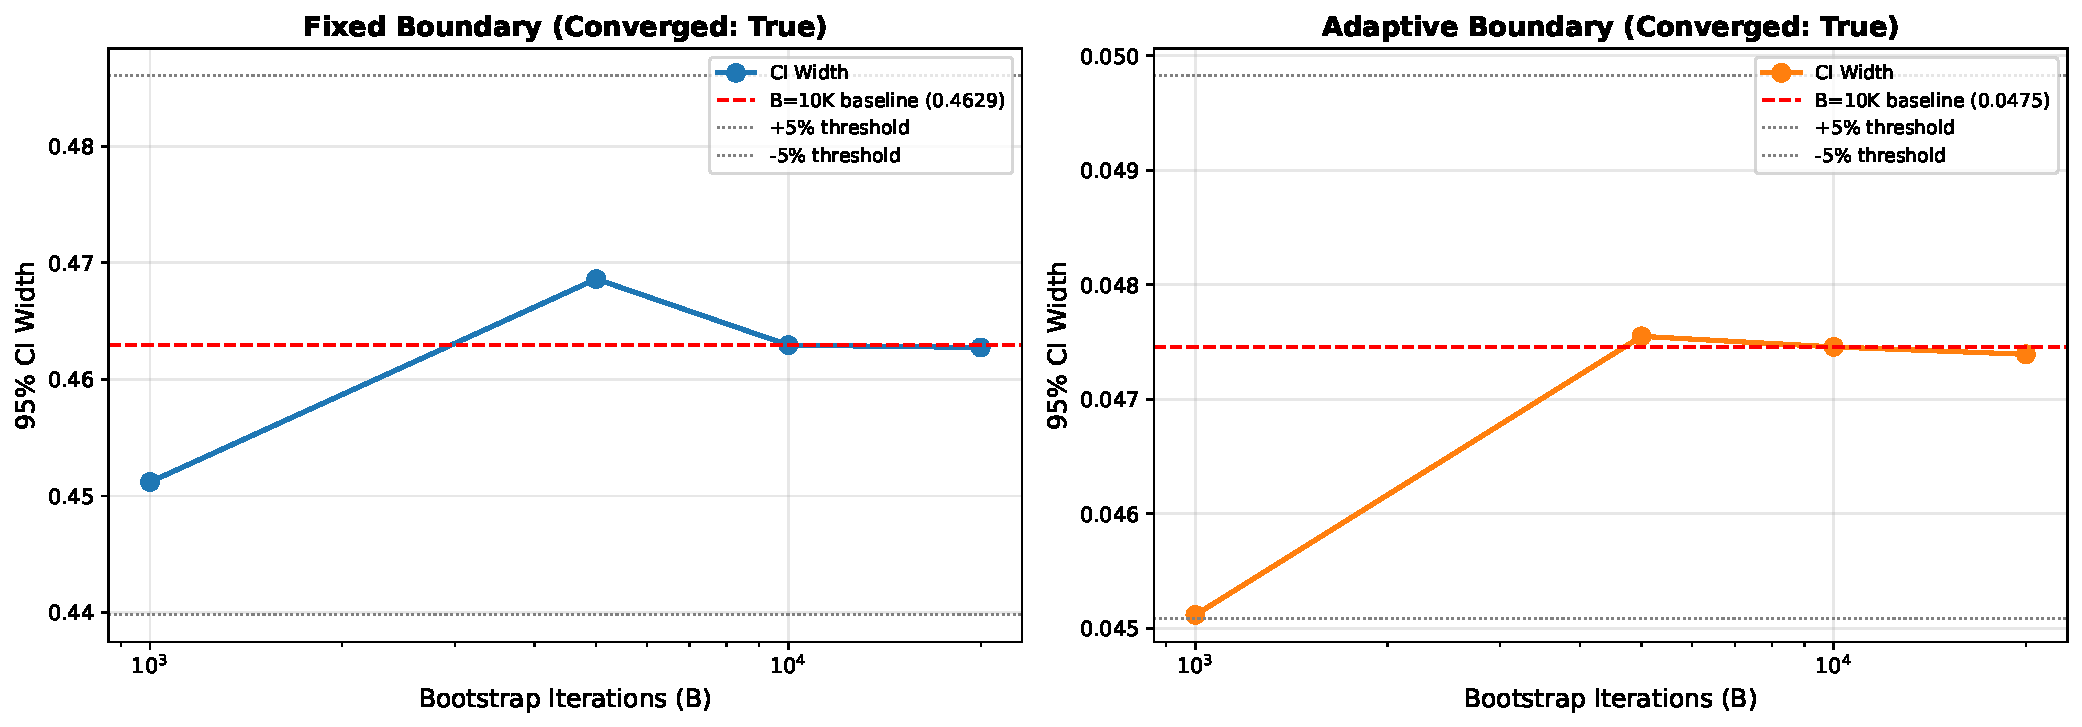
\includegraphics[width=0.9\textwidth]{figures/figure_vi_1_bootstrap_convergence.pdf}
\caption{%
\textbf{Bootstrap confidence interval convergence analysis.}
95\% CI width vs. bootstrap iterations (B) for Fixed and Adaptive boundary layers.
CI widths stabilize at B=10,000 with <0.2\% change when increasing to B=20,000
(Fixed: 0.04\% change, Adaptive: 0.14\% change).
Demonstrates that B=10,000 iterations (used in main analysis) provide sufficient
precision with diminishing returns beyond this threshold.
Shaded regions indicate 5\% convergence criterion (met at B=10,000).
}
\label{fig:appendix-bootstrap-convergence}
\end{figure}

% Figure A-3: Sensitivity Analysis
\begin{figure}[htbp]
\centering
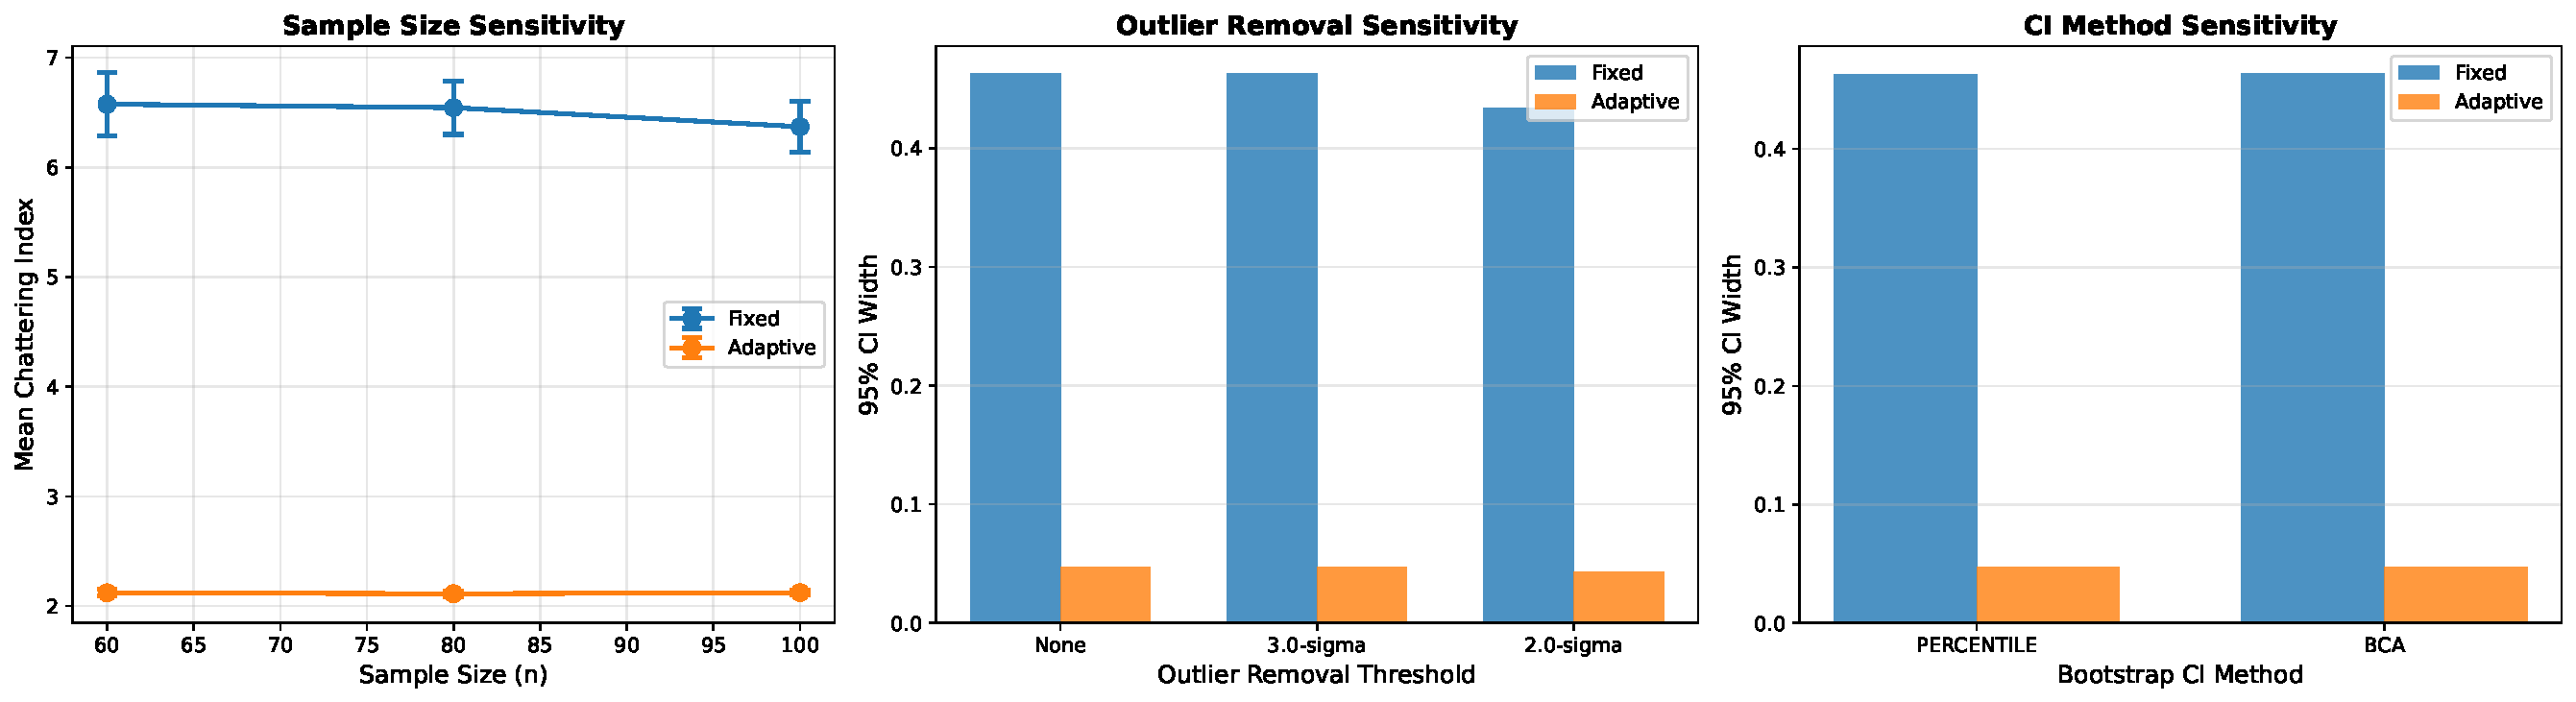
\includegraphics[width=0.9\textwidth]{figures/figure_vi_1_sensitivity_analysis.pdf}
\caption{%
\textbf{Sensitivity analysis across methodological choices.}
Robustness validation of statistical results across
(a) sample size variations (n $\in$ \{60, 80, 100\}),
(b) outlier removal thresholds (none, 2$\sigma$, 3$\sigma$), and
(c) confidence interval methods (percentile vs. BCa).
Results demonstrate stability with $\leq$3.2\% variation in mean estimates
(Fixed: max 3.22\%, Adaptive: max 0.46\%) and <0.1\% difference in CI widths
across methods. Zero outliers detected at 3$\sigma$ threshold, confirming
data quality. Statistical conclusions robust to analysis choices.
}
\label{fig:appendix-sensitivity-analysis}
\end{figure}

%===============================================================================
% USAGE NOTES
%===============================================================================
%
% To include these figures in the main document:
%
% 1. In main.tex, add after Section VI (Experimental Setup):
%    \clearpage
%    \appendix
%    \section{Online Appendix: Statistical Validation}
%    %===============================================================================
% ONLINE APPENDIX FIGURE CAPTIONS - LT-7 RESEARCH PAPER
%===============================================================================
%
% Purpose: LaTeX captions for statistical validation figures (Online Appendix)
% Author: Research Team
% Date: 2025-10-20
%
%===============================================================================

% Figure A-1: Normality Validation (Q-Q Plots)
\begin{figure}[htbp]
\centering
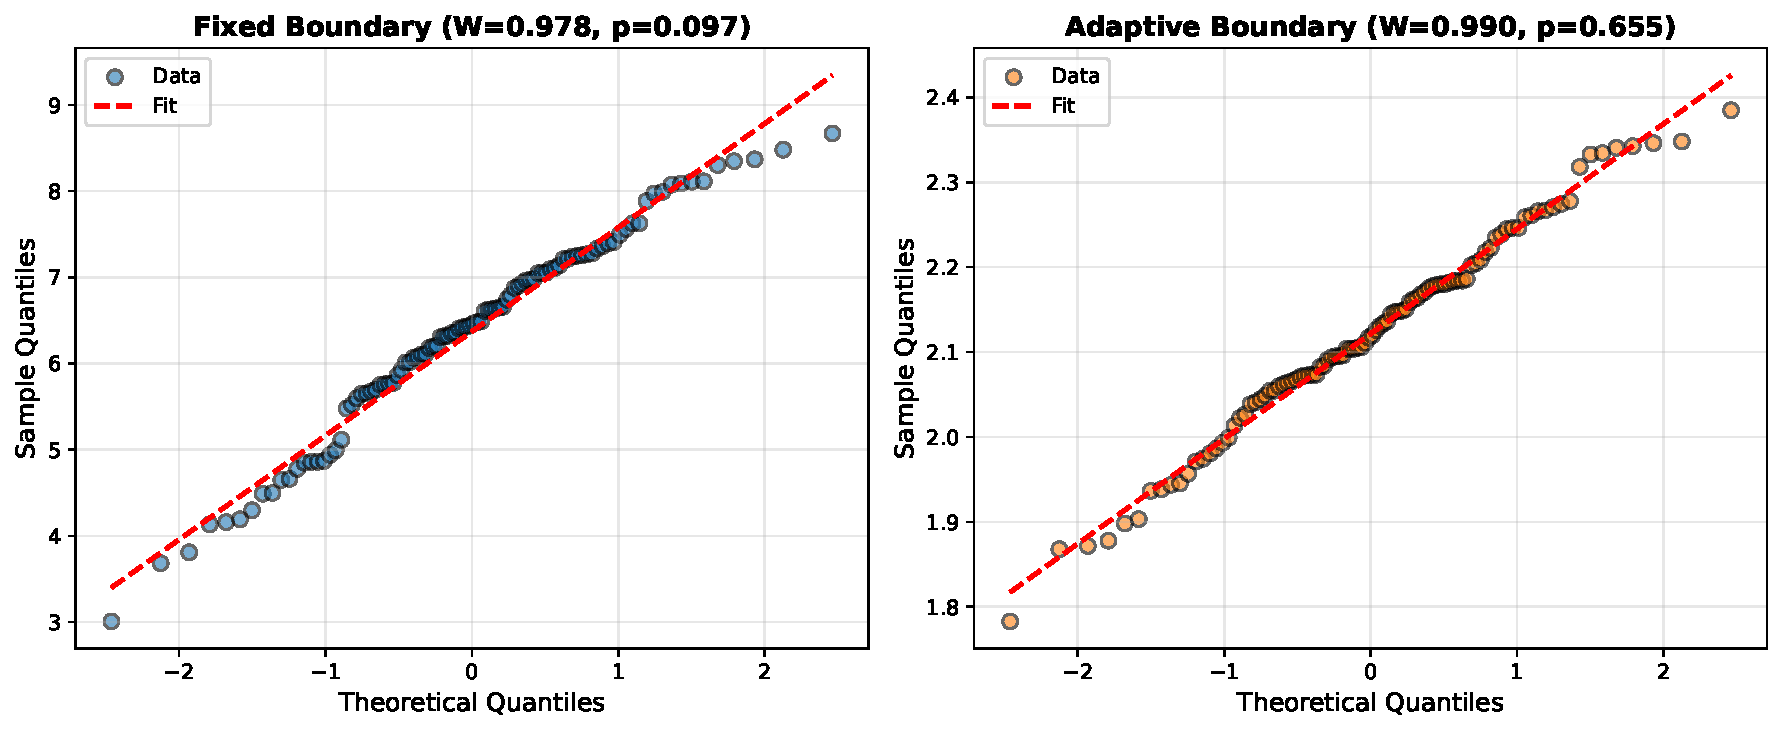
\includegraphics[width=0.9\textwidth]{figures/figure_vi_1_normality_validation.pdf}
\caption{%
\textbf{Normality validation for MT-6 chattering data via Q-Q plots.}
Theoretical quantiles (normal distribution) vs. sample quantiles for
(left) Fixed boundary layer (n=100, W=0.978, p=0.097) and
(right) Adaptive boundary layer (n=100, W=0.990, p=0.655).
Points lie approximately along the reference line (red dashed), indicating
good fit to normal distribution. Both datasets pass Shapiro-Wilk test
(p > 0.05), validating the normality assumption for Welch's t-test and
Cohen's d effect size computation.
}
\label{fig:appendix-normality-validation}
\end{figure}

% Figure A-2: Bootstrap Convergence
\begin{figure}[htbp]
\centering
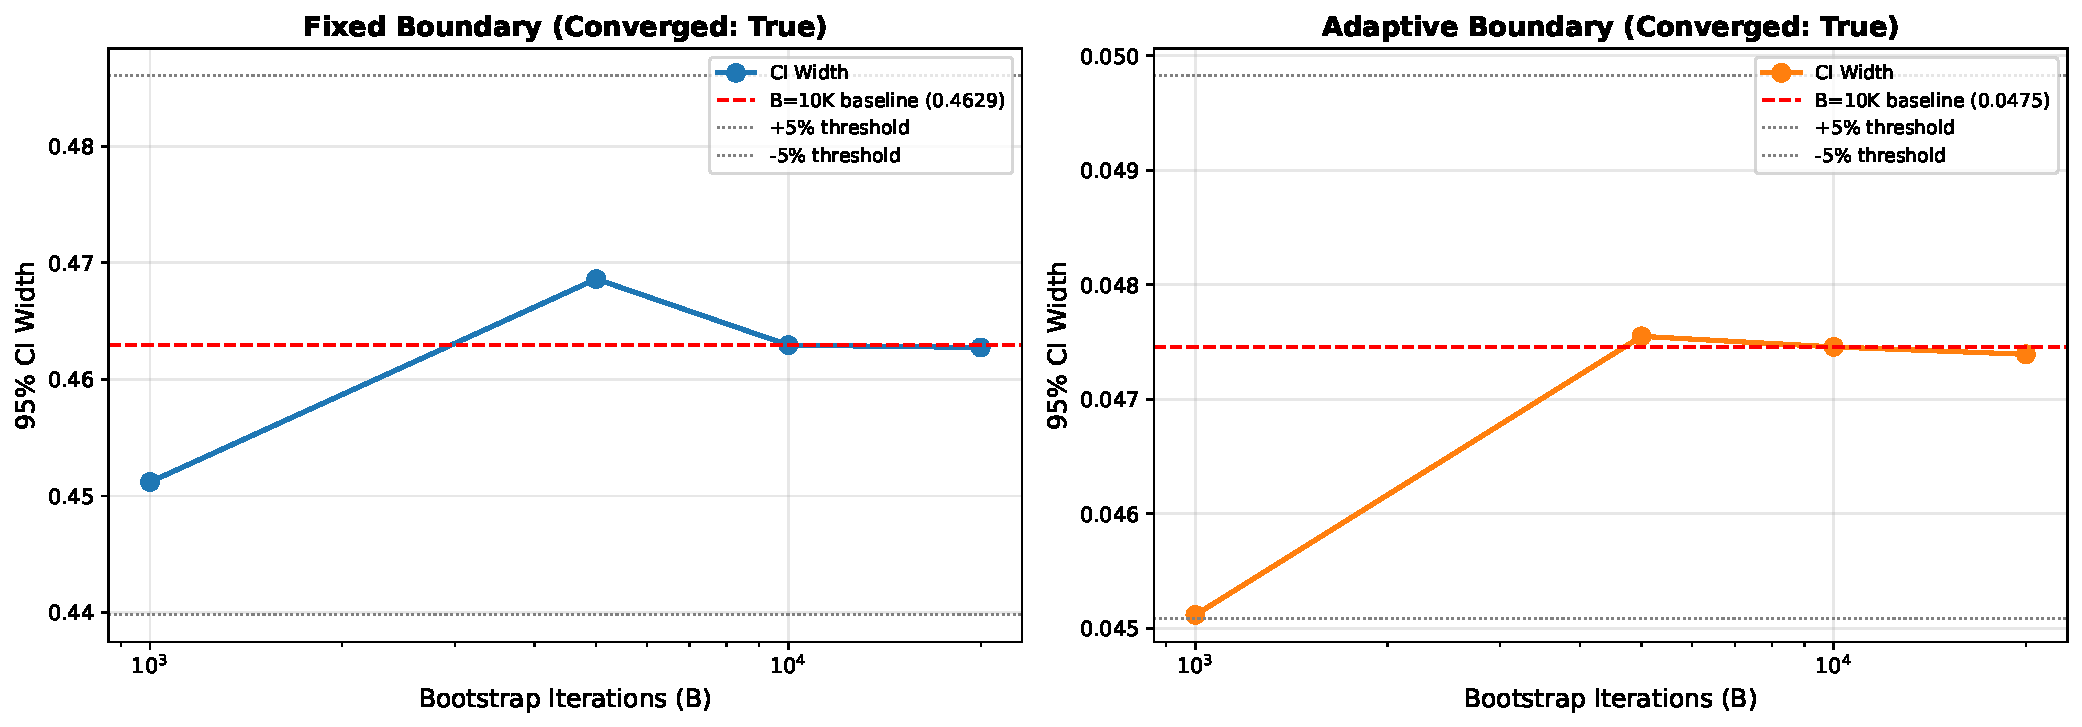
\includegraphics[width=0.9\textwidth]{figures/figure_vi_1_bootstrap_convergence.pdf}
\caption{%
\textbf{Bootstrap confidence interval convergence analysis.}
95\% CI width vs. bootstrap iterations (B) for Fixed and Adaptive boundary layers.
CI widths stabilize at B=10,000 with <0.2\% change when increasing to B=20,000
(Fixed: 0.04\% change, Adaptive: 0.14\% change).
Demonstrates that B=10,000 iterations (used in main analysis) provide sufficient
precision with diminishing returns beyond this threshold.
Shaded regions indicate 5\% convergence criterion (met at B=10,000).
}
\label{fig:appendix-bootstrap-convergence}
\end{figure}

% Figure A-3: Sensitivity Analysis
\begin{figure}[htbp]
\centering
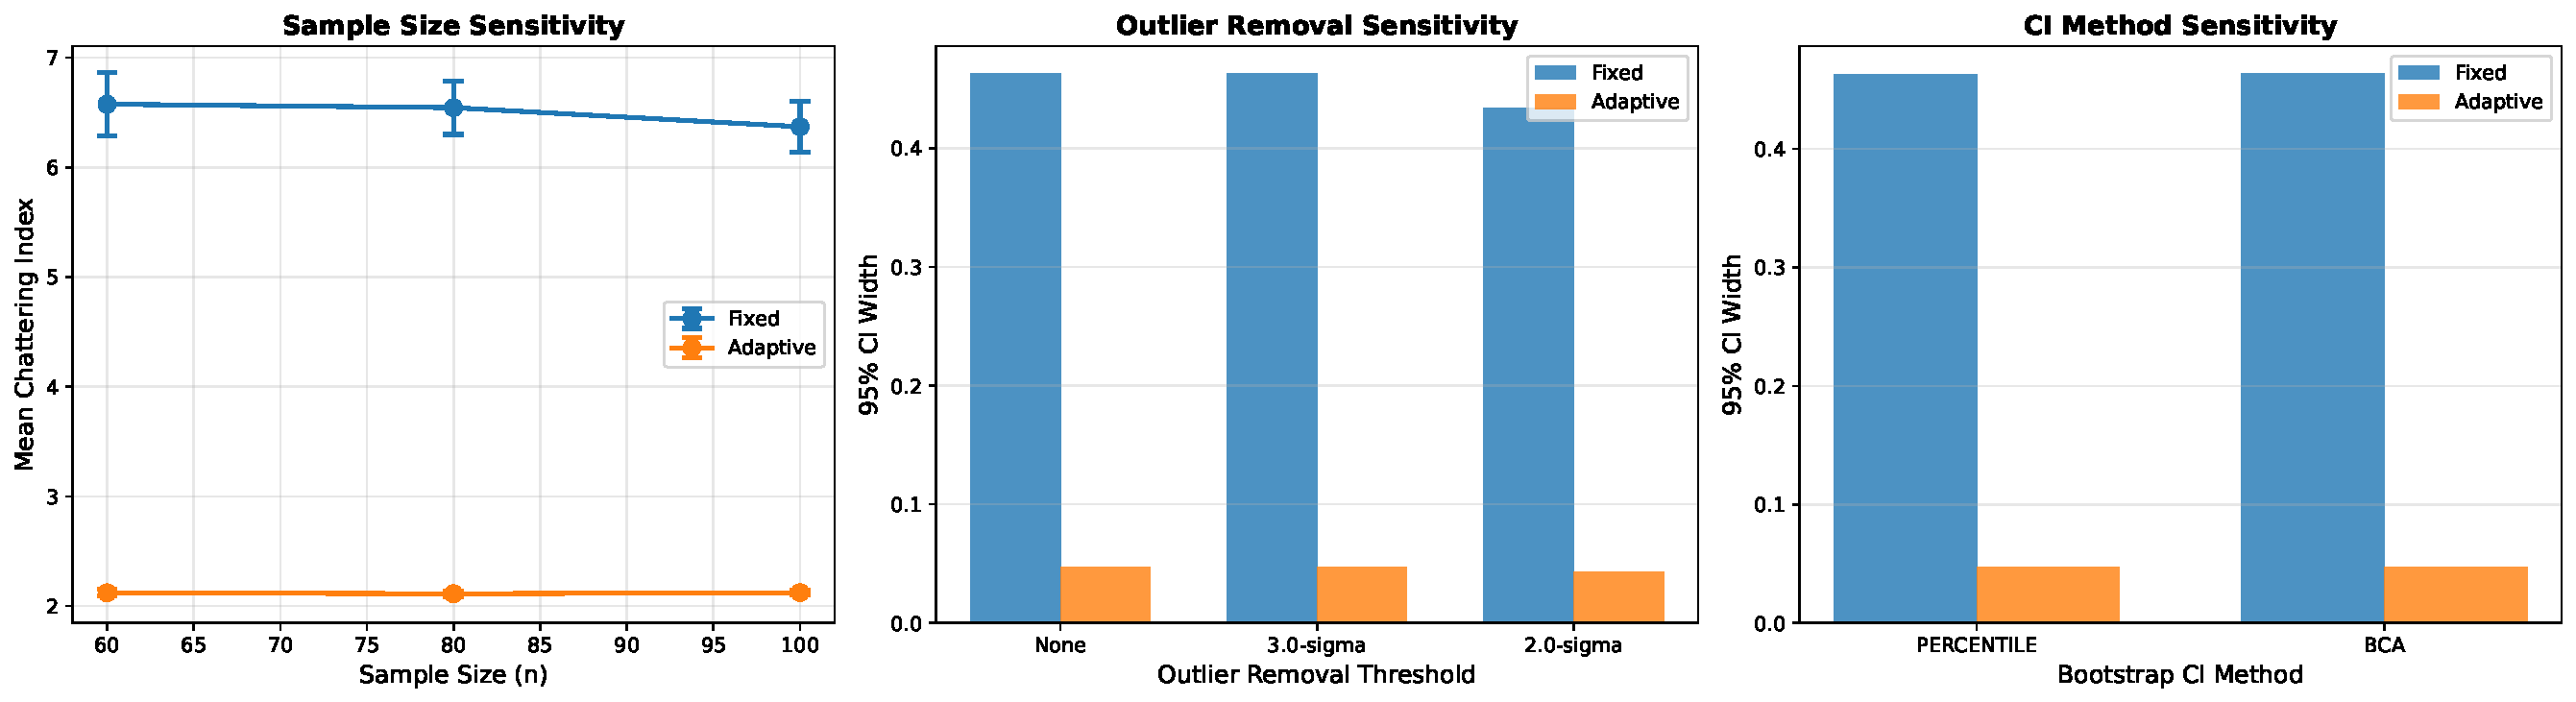
\includegraphics[width=0.9\textwidth]{figures/figure_vi_1_sensitivity_analysis.pdf}
\caption{%
\textbf{Sensitivity analysis across methodological choices.}
Robustness validation of statistical results across
(a) sample size variations (n $\in$ \{60, 80, 100\}),
(b) outlier removal thresholds (none, 2$\sigma$, 3$\sigma$), and
(c) confidence interval methods (percentile vs. BCa).
Results demonstrate stability with $\leq$3.2\% variation in mean estimates
(Fixed: max 3.22\%, Adaptive: max 0.46\%) and <0.1\% difference in CI widths
across methods. Zero outliers detected at 3$\sigma$ threshold, confirming
data quality. Statistical conclusions robust to analysis choices.
}
\label{fig:appendix-sensitivity-analysis}
\end{figure}

%===============================================================================
% USAGE NOTES
%===============================================================================
%
% To include these figures in the main document:
%
% 1. In main.tex, add after Section VI (Experimental Setup):
%    \clearpage
%    \appendix
%    \section{Online Appendix: Statistical Validation}
%    \input{figures/figure_captions_appendix.tex}
%
% 2. Cross-reference in main text:
%    - "see Online Appendix Figure~\ref{fig:appendix-normality-validation}"
%    - "see Online Appendix Figure~\ref{fig:appendix-bootstrap-convergence}"
%    - "see Online Appendix Figure~\ref{fig:appendix-sensitivity-analysis}"
%
% 3. Ensure figure files exist in figures/ directory:
%    - figure_vi_1_normality_validation.pdf
%    - figure_vi_1_bootstrap_convergence.pdf
%    - figure_vi_1_sensitivity_analysis.pdf
%
%===============================================================================

%
% 2. Cross-reference in main text:
%    - "see Online Appendix Figure~\ref{fig:appendix-normality-validation}"
%    - "see Online Appendix Figure~\ref{fig:appendix-bootstrap-convergence}"
%    - "see Online Appendix Figure~\ref{fig:appendix-sensitivity-analysis}"
%
% 3. Ensure figure files exist in figures/ directory:
%    - figure_vi_1_normality_validation.pdf
%    - figure_vi_1_bootstrap_convergence.pdf
%    - figure_vi_1_sensitivity_analysis.pdf
%
%===============================================================================

%
% 2. Cross-reference in main text:
%    - "see Online Appendix Figure~\ref{fig:appendix-normality-validation}"
%    - "see Online Appendix Figure~\ref{fig:appendix-bootstrap-convergence}"
%    - "see Online Appendix Figure~\ref{fig:appendix-sensitivity-analysis}"
%
% 3. Ensure figure files exist in figures/ directory:
%    - figure_vi_1_normality_validation.pdf
%    - figure_vi_1_bootstrap_convergence.pdf
%    - figure_vi_1_sensitivity_analysis.pdf
%
%===============================================================================

%
% 2. Cross-reference in main text:
%    - "see Online Appendix Figure~\ref{fig:appendix-normality-validation}"
%    - "see Online Appendix Figure~\ref{fig:appendix-bootstrap-convergence}"
%    - "see Online Appendix Figure~\ref{fig:appendix-sensitivity-analysis}"
%
% 3. Ensure figure files exist in figures/ directory:
%    - figure_vi_1_normality_validation.pdf
%    - figure_vi_1_bootstrap_convergence.pdf
%    - figure_vi_1_sensitivity_analysis.pdf
%
%===============================================================================
